

Por último existe un lenguaje llamado Elm \cite{evanczaplicki2012:Elm},
creado para poder escribir aplicaciones web reactivas
de una forma funcional declarativa.
  En Elm, las entradas se asumen conocidas y son dadas,
por ejemplo un click o el movimiento del mouse,
o una tecla presionada.

  Todos los valores son señales, el combinador $lift$
toma una señal y una función, y define otra señal resultado
de la aplicación de la función sobre cada valor de la señal.

  Para combinar más de una señal, se usa el combinador $lift_2$ o
$lift_n$ con $n \in N$.
  En los casos que se desea tener memoria, por ejemplo llevar una
cuenta de ocurrencias de una señal, o mantener un estado explícito,
se utiliza el combinador $foldp$.

  El combinador $foldp$ opera sobre una señal como el
operador $fold$ sobre una lista.
  Dado un valor inicial y una función, aplica la función sobre
cada valor, utilizando el último valor conocido como primer argumento.

  La Figura \ref{fig:elmexample} muestra un programa Elm de ejemplo.
  El mismo toma una señal \texttt{Mouse.position}, y dada la función
  \texttt{asText} que convierte un par de valores en texto, utiliza
  \texttt{lift} para aplicar la función a las coordenadas de un Mouse.
 
\begin{figure}[h]
  \begin{center}
  \caption{Ejemplo de programa Elm. (Imagen tomada de \cite{evanczaplicki2012:Elm})}
  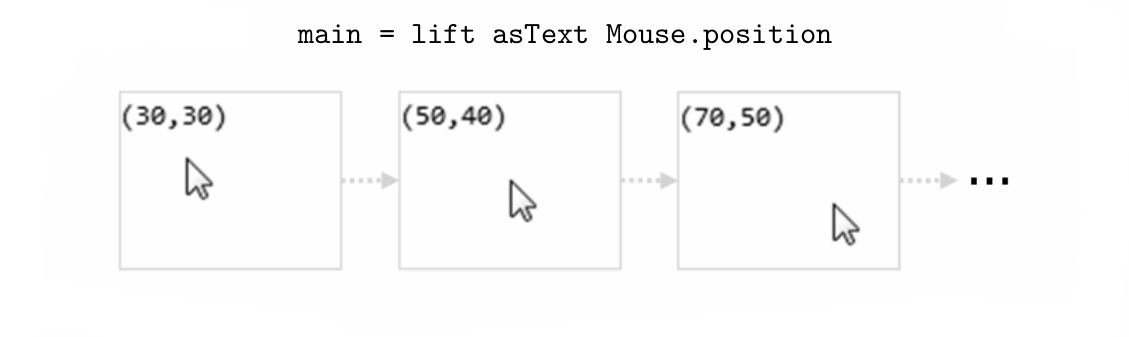
\includegraphics[width=0.9\textwidth]{graphs/elmexample.png}
  \label{fig:elmexample}
  \end{center}
\end{figure}
